\documentclass{article}
\usepackage{amsmath}
\usepackage{mathtools}
\usepackage{gensymb}
\usepackage[a4paper,inner=1.5cm,outer=1.5cm,top=2cm,bottom=0.5cm]{geometry} 
\usepackage{xcolor}                    
\usepackage{tikz}                           
\usepackage{multicol}
\usepackage{hyperref}
\usepackage{pgfplots}
\usetikzlibrary{calc}
\usetikzlibrary{intersections}
\usetikzlibrary{intersections,calc,angles,quotes}
\usetikzlibrary{shapes,arrows,positioning,decorations.pathreplacing,calc}
\usetikzlibrary{calc,angles,positioning,intersections,quotes,decorations.markings}
\usepackage{tkz-euclide}
\usetikzlibrary{backgrounds}
\usetikzlibrary{calc,through}
\usetikzlibrary{angles}
\usetikzlibrary{fadings}
\usetikzlibrary{shapes.geometric}
\usetikzlibrary{shapes.symbols}
\usepackage{draftwatermark}
\usepackage{mathptmx}

\SetWatermarkText{\textcolor{black!20}{Mathema Shukur}}
\SetWatermarkFontSize{2 cm}
\usepackage[utf8]{inputenc}
\usepackage{fontspec}

\setmainfont{[Kalpurush.ttf]}
\newfontface{\en}{[Arial.ttf]} %%this is optional, if you want to use a secondary font. Any english font is supported
\newlength\Radius
\setlength\Radius{4cm}
\begin{document} 
	\Large
	\textcolor{red}{Welcome To} 
	\\
	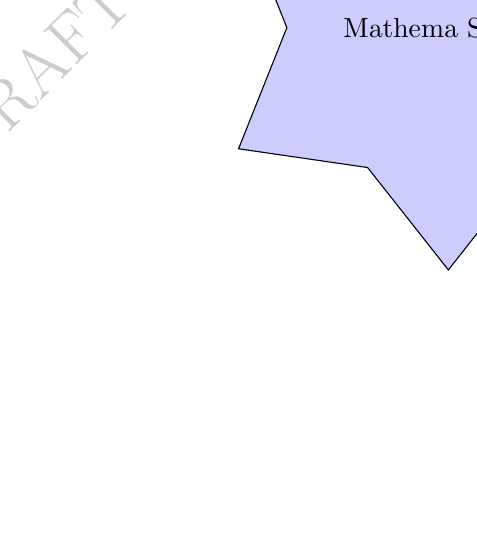
\begin{tikzpicture}
		\tikz \node [fill=blue!20,star,star points=6,draw] {Mathema Shukur };
	\end{tikzpicture}
	\\
	যাদের জন্যে প্রযোজ্যঃ  	\textcolor{magenta}{একাদশ ও দ্বাদশ শ্রেণীর শিক্ষার্থী} \\
	বিষয়ঃ \textcolor{magenta}{উচ্চতর গণিত ১ম পত্র} \\
	অধ্যায়ঃ \textcolor{magenta}{৪-বৃত্ত}\\ 
	\\
	\\
	\href{https://www.youtube.com/watch?v=DRxNte3mU6U&list=PLIjPH8h-K22w5iYZogyV1AI8-baSpY2Qn&index=1}{\textcolor{blue}{মূল বিন্দুতে (0,0) কেন্দ্র থাকলে বৃত্তের সমীকরণ কী?}}\\
	\\
	\href{https://www.youtube.com/watch?v=rGCA1MltZsY&list=PLIjPH8h-K22w5iYZogyV1AI8-baSpY2Qn&index=2}{\textcolor{blue}{কী শর্তে কেন্দ্রের স্থানাঙ্ক হতে বৃত্তের ব্যাসার্ধ নির্ণয় করা হয়?}}\\
	\\
	\href{https://www.youtube.com/watch?v=gehIW-_0XrQ&list=PLIjPH8h-K22w5iYZogyV1AI8-baSpY2Qn&index=3}{\textcolor{blue}{বৃত্তের সাধারণ সমীকরণ $x^2+y^2+2gx+2fy+c=0$}}\\
	\\
	\href{https://www.youtube.com/watch?v=WzuG-MuA6Cs&list=PLIjPH8h-K22w5iYZogyV1AI8-baSpY2Qn&index=4}{\textcolor{blue}{পোলার স্থানাঙ্কে বৃত্তের সমীকরণ নির্ণয়}}\\
	\\
	\href{https://www.youtube.com/watch?v=ssCuBx7HEHI&list=PLIjPH8h-K22w5iYZogyV1AI8-baSpY2Qn&index=5}{\textcolor{blue}{ব্যাসের প্রান্ত বিন্দু (x1,y1) ও (x2,y2) হলে বৃত্তের সমীকরণ নির্ণয়}}\\
	\\
	\href{https://www.youtube.com/watch?v=afVjGQrIpDs&list=PLIjPH8h-K22w5iYZogyV1AI8-baSpY2Qn&index=6}{\textcolor{blue}{বৃত্ত ও সরলরেখার ছেদবিন্দুগামী বৃত্তের সমীকরণ}}\\
	\\
	\href{https://www.youtube.com/watch?v=rXOyjYE6YfU&list=PLIjPH8h-K22w5iYZogyV1AI8-baSpY2Qn&index=7}{\textcolor{blue}{দুইটি বৃত্তকে ছেদ করে এমন বৃত্তের সমীকরণ}}\\
	\\
	\href{https://www.youtube.com/watch?v=iQIWTRqZsAY}{\textcolor{blue}{৩ টি বিন্দুগামী বৃত্তের সমীকরণ নির্ণয়}}\\
		\\
	\href{https://www.youtube.com/watch?v=zsiv_hlMIR0}{\textcolor{blue}{২ টি বৃত্ত পরস্পরকে স্পর্শ করার শর্ত}}\\
	\\
	\textcolor{magenta}{একটি সরলরেখা বৃত্তের স্পর্শক হওয়ার শর্ত }\\
	\\
	বৃত্তের কেন্দ্র হতে রেখাটির লম্ব দূরত্ব বৃত্তের ব্যাসার্ধের সমান হলে রেখাটি বৃত্তকে স্পর্শ করবে।\\
	\\ 
		\\
\textcolor{green}{$3x+2y+k=0$ রেখাটি  $x^2+y^2-8x-2y+4=0$ বৃত্তকে স্পর্শ করলে $k$ এর মান  নির্ণয় কর।}\\
	\\
	\begin{align*}
		x^2+y^2-8x-2y+4&=0\\
		\boxed{\textcolor{blue}{x^2+y^2+2gx+2fy+c=0}}&\\
		x^2+y^2+2(-4)x+2(-1)y+4&=0
	\end{align*}
	\\
	কেন্দ্র 	$(-g,-f)=(4,1)$ ও ব্যাসার্ধ= $\sqrt{g^2+f^2-c}=\sqrt{(-4)^2+(-1)^2-4}=\sqrt{13}=r$\\
	\\ 
	\textcolor{blue}{$P(x_1,y_1)$ বিন্দু হতে  $ax+by+c=0$ সরলরেখার উপর অঙ্কিত লম্বের দৈর্ঘ্য বা লম্ব দূরত্ব \\
		\\
		$d=\frac{|ax_1+by_1+c|}{\sqrt{a^2+b^2}}$}\\
	\\
	কেন্দ্র \textcolor{green}{$(4,1)$} হতে \textcolor{magenta}{$3x+2y+k=0$}  রেখার লম্ব দূরত্ব \\
	\begin{align*}
		d=	&\frac{|3(4)+2(1)+k|}{\sqrt{3^2+2^2}}\\
		\\
		=	&	\frac{|14+k|}{\sqrt{13}}\\
	\end{align*}
\\
	\begin{tikzpicture}[transform shape,scale=1]
		\draw[thick,green] (4,1) circle (3.60);
		\fill[green] (4,1) circle (1 mm);
		\draw[magenta,dashed](4,1)--(1,-1);
		\draw[magenta](-1,2)--(3,-4);
	\end{tikzpicture}\\
	\\ 
	\begin{align*}
		d&=r\\
		\\
		\frac{|14+k|}{\sqrt{13}}&=\sqrt{13}	\\
		\\
		|14+k|&=13\\
		\\
		14+k&=\pm 13\\
		\\
		k&=\pm13-14\\
		\\
		k&=-1,\,\,-27
	\end{align*}
\\ 
$k=-1$ হলে সরলরেখাটি হবে  \textcolor{magenta}{$3x+2y-1=0$}\\
\\
$k=-27$ হলে সরলরেখাটি হবে  \textcolor{cyan}{$3x+2y-27=0$}\\
\\ 
	\begin{tikzpicture}[transform shape,scale=1]
	\draw[thick,green] (4,1) circle (3.60);
	\fill[green] (4,1) circle (1 mm);
	\draw[magenta,dashed](4,1)--(1,-1);
	\draw[magenta](-1,2)--(3,-4);
	\draw[cyan](5,6)--(11,-3); 
	\draw[cyan,dashed](4,1)--(7,3);
\end{tikzpicture}\\
	\\
অনুশীলন-১ঃ  $x+y=1$ রেখাটি  $x^2+y^2-2ax=0$ বৃত্তকে স্পর্শ করার শর্ত নির্ণয় কর। \\
	\\
অনুশীলন-২ঃ  $3x+ky-1=0$ রেখাটি  $x^2+y^2-8x-2y+4=0$ বৃত্তকে স্পর্শ করলে $k$ এর মান  নির্ণয় কর। \\
		\\
		\\
		\\
		\\ 
	\textcolor{green}{$y=mx+c$ রেখাটি  $x^2+y^2=a^2$ বৃত্তকে স্পর্শ করার শর্ত নির্ণয় কর।} \\
		\\
		$y=mx+c$ এবং   $x^2+y^2=a^2$ 	সমীকরণটি সমাধান করি\\ 
		\\ 
		\begin{align*}
			x^2+y^2&=a^2\\
			\\
			x^2+(mx+c)^2&=a^2\,\,\,\boxed{\textcolor{blue}{y=mx+c}}\\
			\\
			x^2+m^2\,\,x^2+2\,\,mx\,\,c+c^2-a^2&=0\\
			\\
			(1+m^2)x^2+2\,\,m\,\,c\,\,x+(c^2-a^2)&=0
		\end{align*}
	\\ 
রেখাটি বৃত্তের স্পর্শক হলে $	(1+m^2)x^2+2\,\,m\,\,c\,\,x+(c^2-a^2)=0$ দ্বিঘাত সমীকরণের একটি মূল থাকবে অর্থাৎ মূলদ্বয় সমান হবে। \\
\\
মূল দুইটি সমান হবার শর্ত , পৃথায়কের মান  শূন্য হবে \\
\\
	\textcolor{cyan}{[ $a_1x^2+b_1x+c_1=0$ দ্বিঘাত সমীকরণের পৃথায়ক $D=b_1^2-4\,\,a_1\,\,c_1$]}\\
\\ 
	$a_1=(1+m^2)$,\,\,\, $b_1=2\,\,m\,\,c$,\,\,\, $c_1=c^2-a^2$\\
	\\
	\begin{align*}
		D&=b_1^2-4\,\,a_1\,\,c_1\\
		\\
		&=(2\,\,m\,\,c)^2-4\,\,(1+m^2)\,\,(c^2-a^2)\\
		\\
		&=4\,\,m^2\,\,c^2-4\,\,(1+m^2)\,\,(c^2-a^2)\\
		\\
		&=4[m^2\,\,c^2-c^2-m^2\,\,c^2+m^2\,\,a^2+a^2]\\
		\\
		&=4[a^2(1+m^2)-c^2]
	\end{align*}
\\
মূল দুইটি সমান হবার শর্ত , পৃথায়কের মান  শূন্য হবে \\
\\
	\begin{align*}
4[a^2(1+m^2)-c^2]&=0\\
\\
a^2(1+m^2)-c^2&=0\\
\\
c^2&=a^2(1+m^2)\\
\\
c&=\pm \sqrt{a^2(1+m^2)}\\
\\
c&=\pm a\sqrt{1+m^2}
\end{align*}
\\
$y=mx+c$ রেখাটি  $x^2+y^2=a^2$ বৃত্তকে স্পর্শ করার শর্ত  $c=\pm a\sqrt{1+m^2}$\\
\\ 
অনুশীলন-৩ঃ  $c$ এর মান কত হলে  $y=3x+c$ সরলরেখাটি $x^2+y^2=10$ বৃত্তকে স্পর্শ করবে। \\
\\
অনুশীলন-৪ঃ   $c$ এর মান কত হলে  $y=c$ সরলরেখাটি $x^2+y^2=4$ বৃত্তকে স্পর্শ করবে। \\
\end{document}